%!TEX root = pset1.tex

\section{Implement Gradient Descent}\label{sec:grad_desc}

\subsection{Implementation}
We implemented a basic gradient descent function in MATLAB. In this function, the user can specify the objective function and the corresponding gradient function. User also specify initial guess, the constant step size, and the convergence threshold. \\
The procedure works as the following: starting at the initial guess, we move to a new point by taking a step (of the specified step size) in the direction of the gradient. We repeat the process until the objective values between two iterations are less than the specified threshold.

\subsection{Testing Gradient Descent}
We test the gradient descent procedure in the following functions:
\begin{enumerate}
\item $f(x_1, x_2) = 3x_1^2 + 2x_1x_2 + x_2^2 - 4x_1 + 5x_2$ (By completing the square we get the optimal value is at $x_1 = 2.25, x_2 = -4.75$.)
\item $f(x) = -\frac{1}{\sqrt{2\pi}\sigma}e^{-(x-\mu)^2/2\sigma^2}$ (negative of a Gaussian pdf, with $\mu = 0$ and $\sigma = 1$.)
\item $f(x) = x^3 - 10x$. (This is not a convex function; local minimum is at $1.8257$ and global minimum is negative infinity).
\end{enumerate}

The basic gradient descent method works decently well in the first two functions. In most specifications of the initial guess and step size the procedure converges to the right answer. Changing the convergence threshold to very large gives imprecise results, and changing it to very small results in more iterations until convergence. In some cases, very large or very small step sizes may result in non-convergence. In the third function which is non-convex, the initial guess can lead us to the incorrect, local minimum.  

\begin{figure}[h!]
\centering
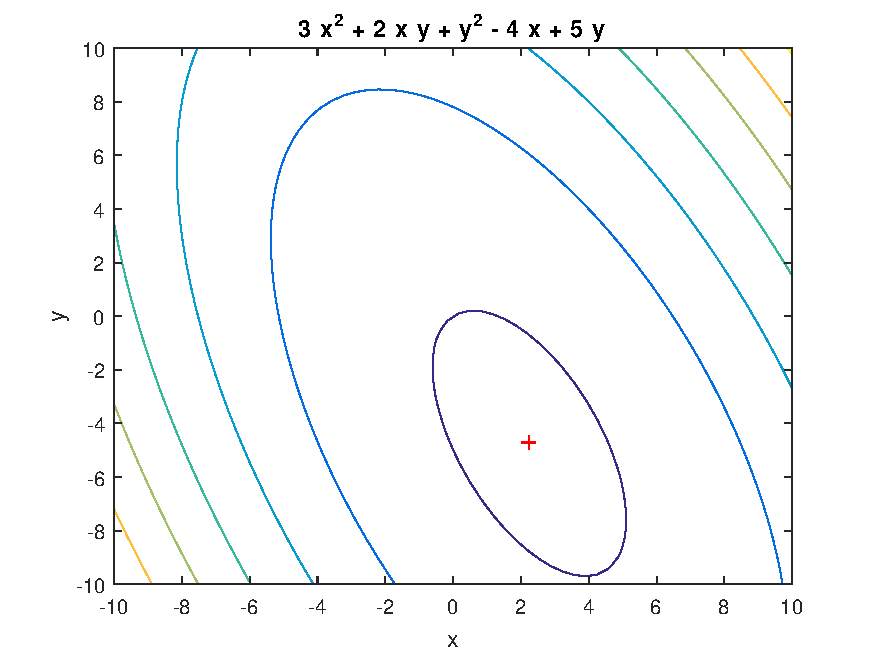
\includegraphics[scale=0.4]{hw1_1.pdf}
\caption{Contour plot of the first function. The gradient descent method moves along the red dots in the steps toward the red cross where the local/global optimal is.}
\end{figure}


\subsection{Numerical Gradient}
We can also numerically evaluate the gradient at a given point. The partial derivative at $x_i$ is evaluated by taking the difference between $f(\V x+\V h)$ and $f(\V x-\V h)$, where $\V h$ is the vector of all zeros except for the $i$th component being $\epsilon$, and divide the difference by $2\epsilon$. We apply this numerical gradient in place of the analytic one in the original three functions, and found that for sufficiently small $\epsilon$, the results are almost identical!

\subsection{Comparing with Sophisticated Methods}
As the final step to evaluate our implementation of gradient descent, we would like to compare ours with the more developed methods. Comparing with \texttt{fminunc}, our implementation is dramatically slower, unfortunately. For example, for the same convergence criterion, it takes 8 iterations for \texttt{fminunc} to converge, whereas it takes 35 iterations for our method. We think the disadvantage is from our constant step size. Since this size does not adapt to where we are, our method is likely to undershoot or overshoot. An improvement could be using backtracking, exact line-search, etc. methods to adaptively update the step size.  